\documentclass[conference]{IEEEtran}
\IEEEoverridecommandlockouts
% The preceding line is only needed to identify funding in the first footnote. If that is unneeded, please comment it out.
\usepackage{cite}
\usepackage{amsmath,amssymb,amsfonts}
\usepackage{graphicx}
\usepackage{textcomp}
\usepackage{xcolor}
\def\BibTeX{{\rm B\kern-.05em{\sc i\kern-.025em b}\kern-.08em
    T\kern-.1667em\lower.7ex\hbox{E}\kern-.125emX}}
\title{
\vspace{1cm}
{
\includegraphics[width=0.15\textwidth]{ /storage/emulated/0/vignan/IMG-20241018-WA0001.jpg} \\ ESP Assignment}}
\author{Bynaboyina Aiswarya \\ Roll No: FWC22295 \\ aiswaryabaiswarya61@gmail.com}
 \begin{document}
\maketitle
 \section{ABSTRACT}

This paper explains about determining the logic values \( X_2 \) and \( Y_2 \) for a given digital circuit by analyzing its truth table and circuit diagram. The circuit consists of multiple logic gates (AND, OR, and NOT gates) connected in a specific configuration, with inputs labeled \( G \), \( A \), \( B \), \( P \), and \( C \). By evaluating the output of each gate based on the inputs, the values of \( X \) and \( Y \) are derived and matched against the truth table. This approach allows us to accurately identify the correct logic values for \( X_2 \) and \( Y_2 \).


\begin{figure}[h]                         
\centering                                
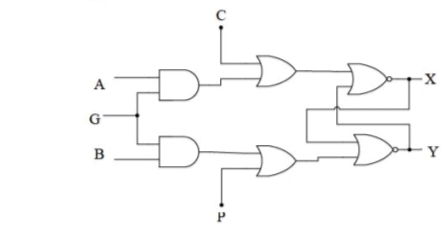
\includegraphics[width=0.4\textwidth]{ /storage/emulated/0/vignan/IMG_20241028_122518.jpg }                               
\caption{\label{fig-1:Gates}}             
\end{figure}

\begin{figure}[h]                       
\centering                               
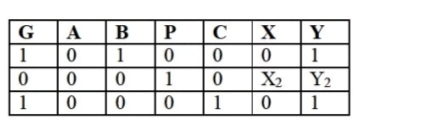
\includegraphics[width=0.4\textwidth]{ /storage/emulated/0/vignan/IMG_20241028_122658.jpg }                                
\caption{\label{fig-2:Gates}}             
\end{figure}


\section{COMPONENTS} 

The required components list is given in Table: I., pin diagram of vaman is shown in Fig.1.
\vspace{0.3cm}
 \begin{table} [htbp]
\centering
\begin{tabular}{| c | c |} \hline
Components  & Quantity \\\hline
vaman   & 1 \\ \hline
led  & 2 \\ \hline
Jumper Wires   & 10 \\ \hline
Breadboard & 1 \\ 
\hline
\end{tabular}
\vspace{0.1cm}
\caption{\label{tab:widgets}}
\end{table}

\section{PROCEDURE}
 \begin{enumerate}
\item Pin Configuration of vaman board.

\begin{figure}[h]                           
\centering                                 
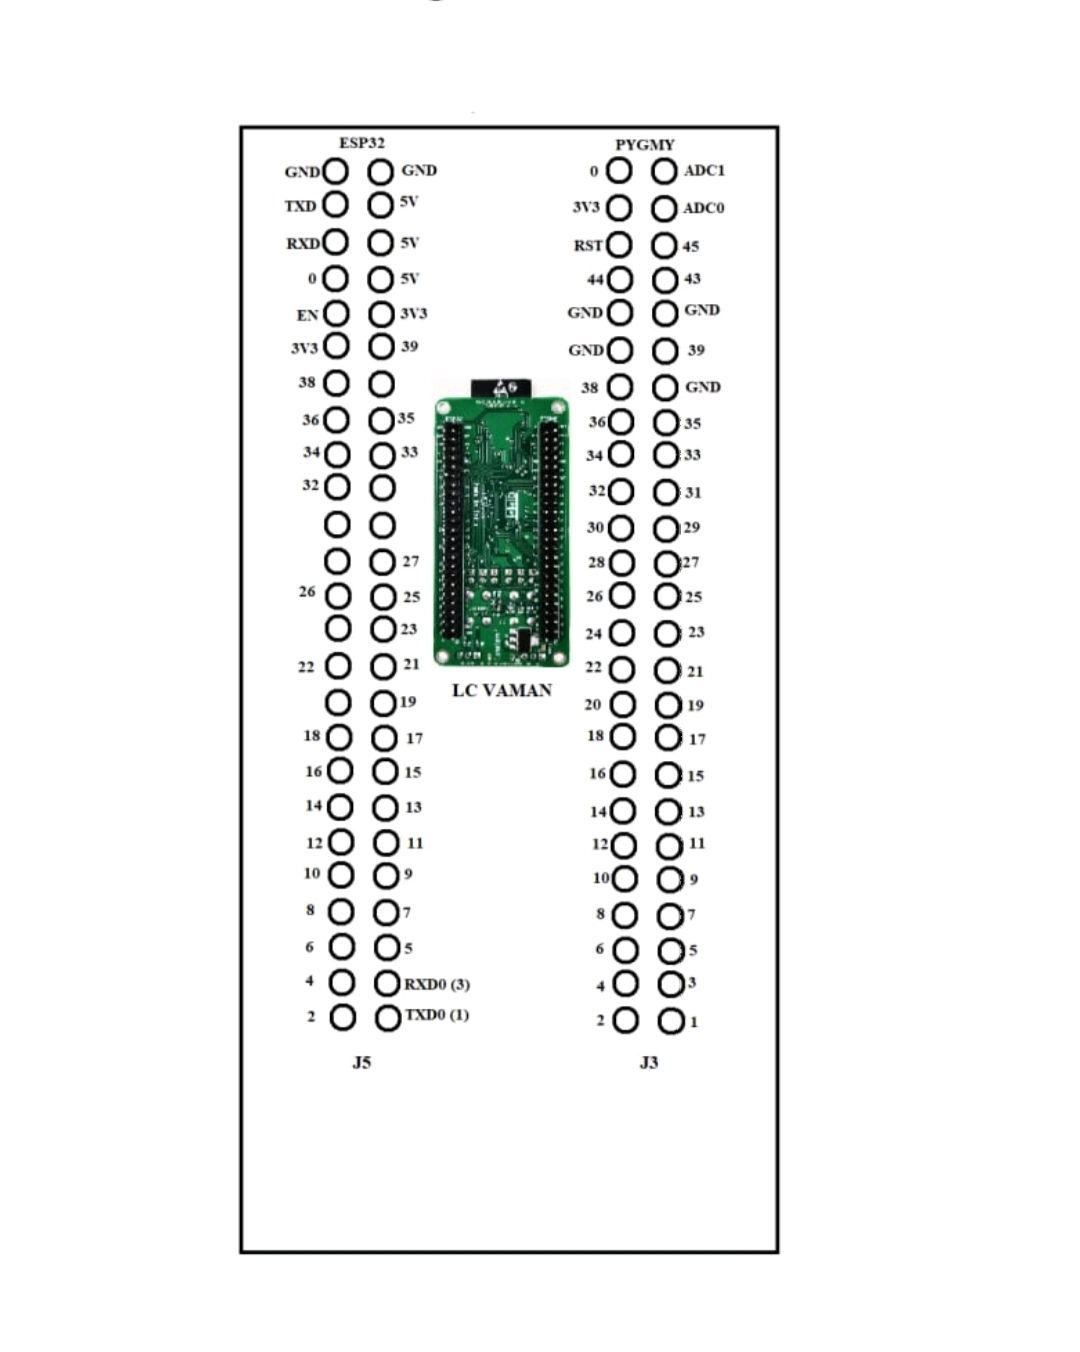
\includegraphics[width=0.3\textwidth]{/storage/emulated/0/vignan/IMG_20241028_124035.jpg	}                                           
\caption{\label{fig-3:Gates}}               
\end{figure}

\item Make connections of vaman to two leds as per below table.

\begin{table} [htbp]
\centering
\begin{tabular}{| c | c | c |} \hline
Led-1 & Led-2 & Vaman \\\hline
Anode & - & GPIO-2 \\ \hline
 -  & Anode & GPIO-4 \\ \hline
Cathode & Cathode  & Gnd \\  
\hline
\end{tabular}
\vspace{0.1cm}
\caption{\label{tab:widgets}}
\end{table}


\item Execute the esp code with wifi in nvim editor using the command called pio run.
\item After upload the esp-code into hardware setup using the command called pio run -t nobuild -t upload --upload-port 192.168.217.128.
\begin{figure}[h]                       
\centering                               
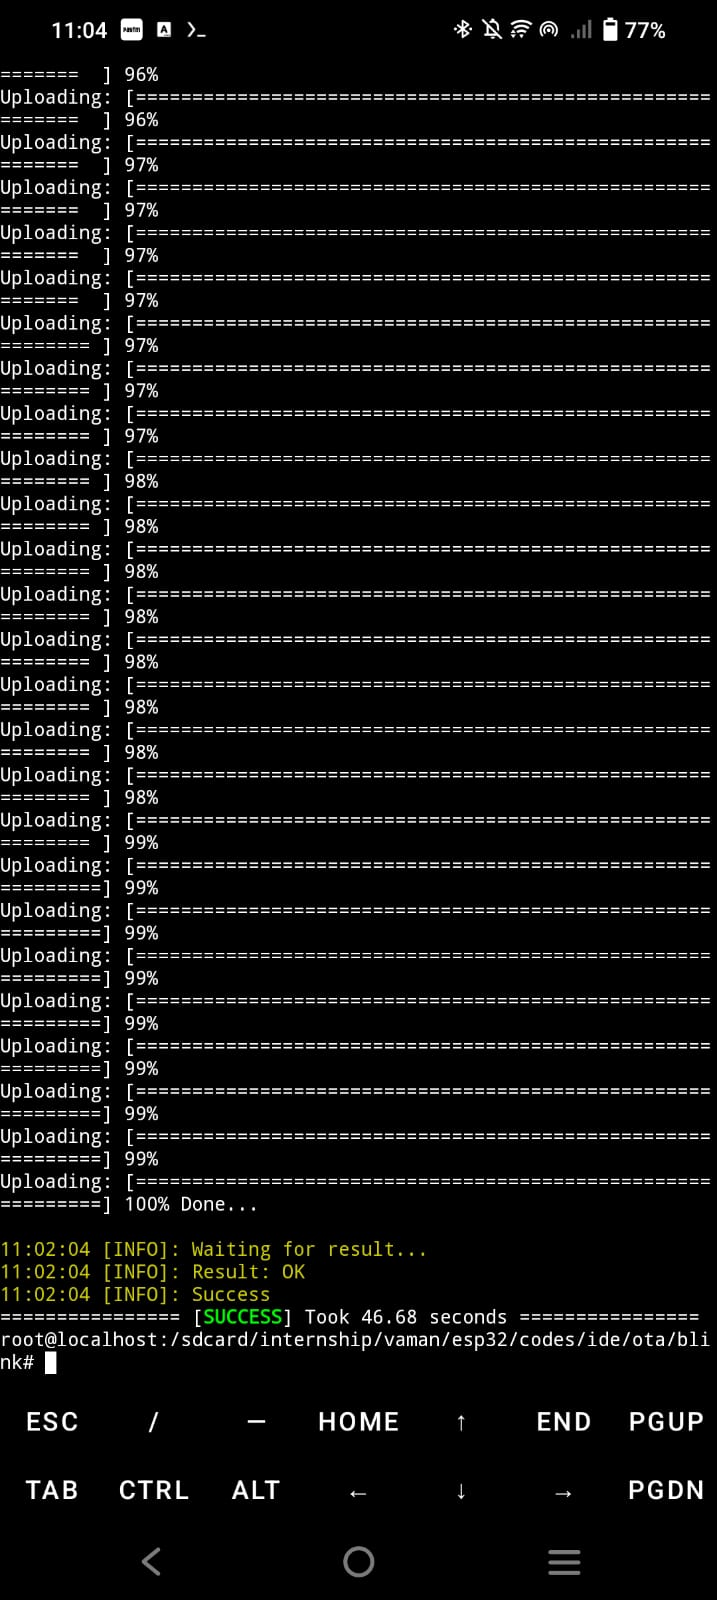
\includegraphics[width=0.2\textwidth]{ /storage/emulated/0/vignan/IMG-20241028-WA0003.jpg	}                                
\caption{\label{fig-4:Gates}}             
\end{figure}


 \end{enumerate}

\section{RESULTS}
 \begin{enumerate}
\item Download the codes given in the link below and execute them to see the output as shown in figure 3.
\item https://github.com/BynaboyinaAiswarya/Fwc-/blob/main/Esp/main.cpp
 \end{enumerate}

 \begin{figure}[h]                       
\centering                               
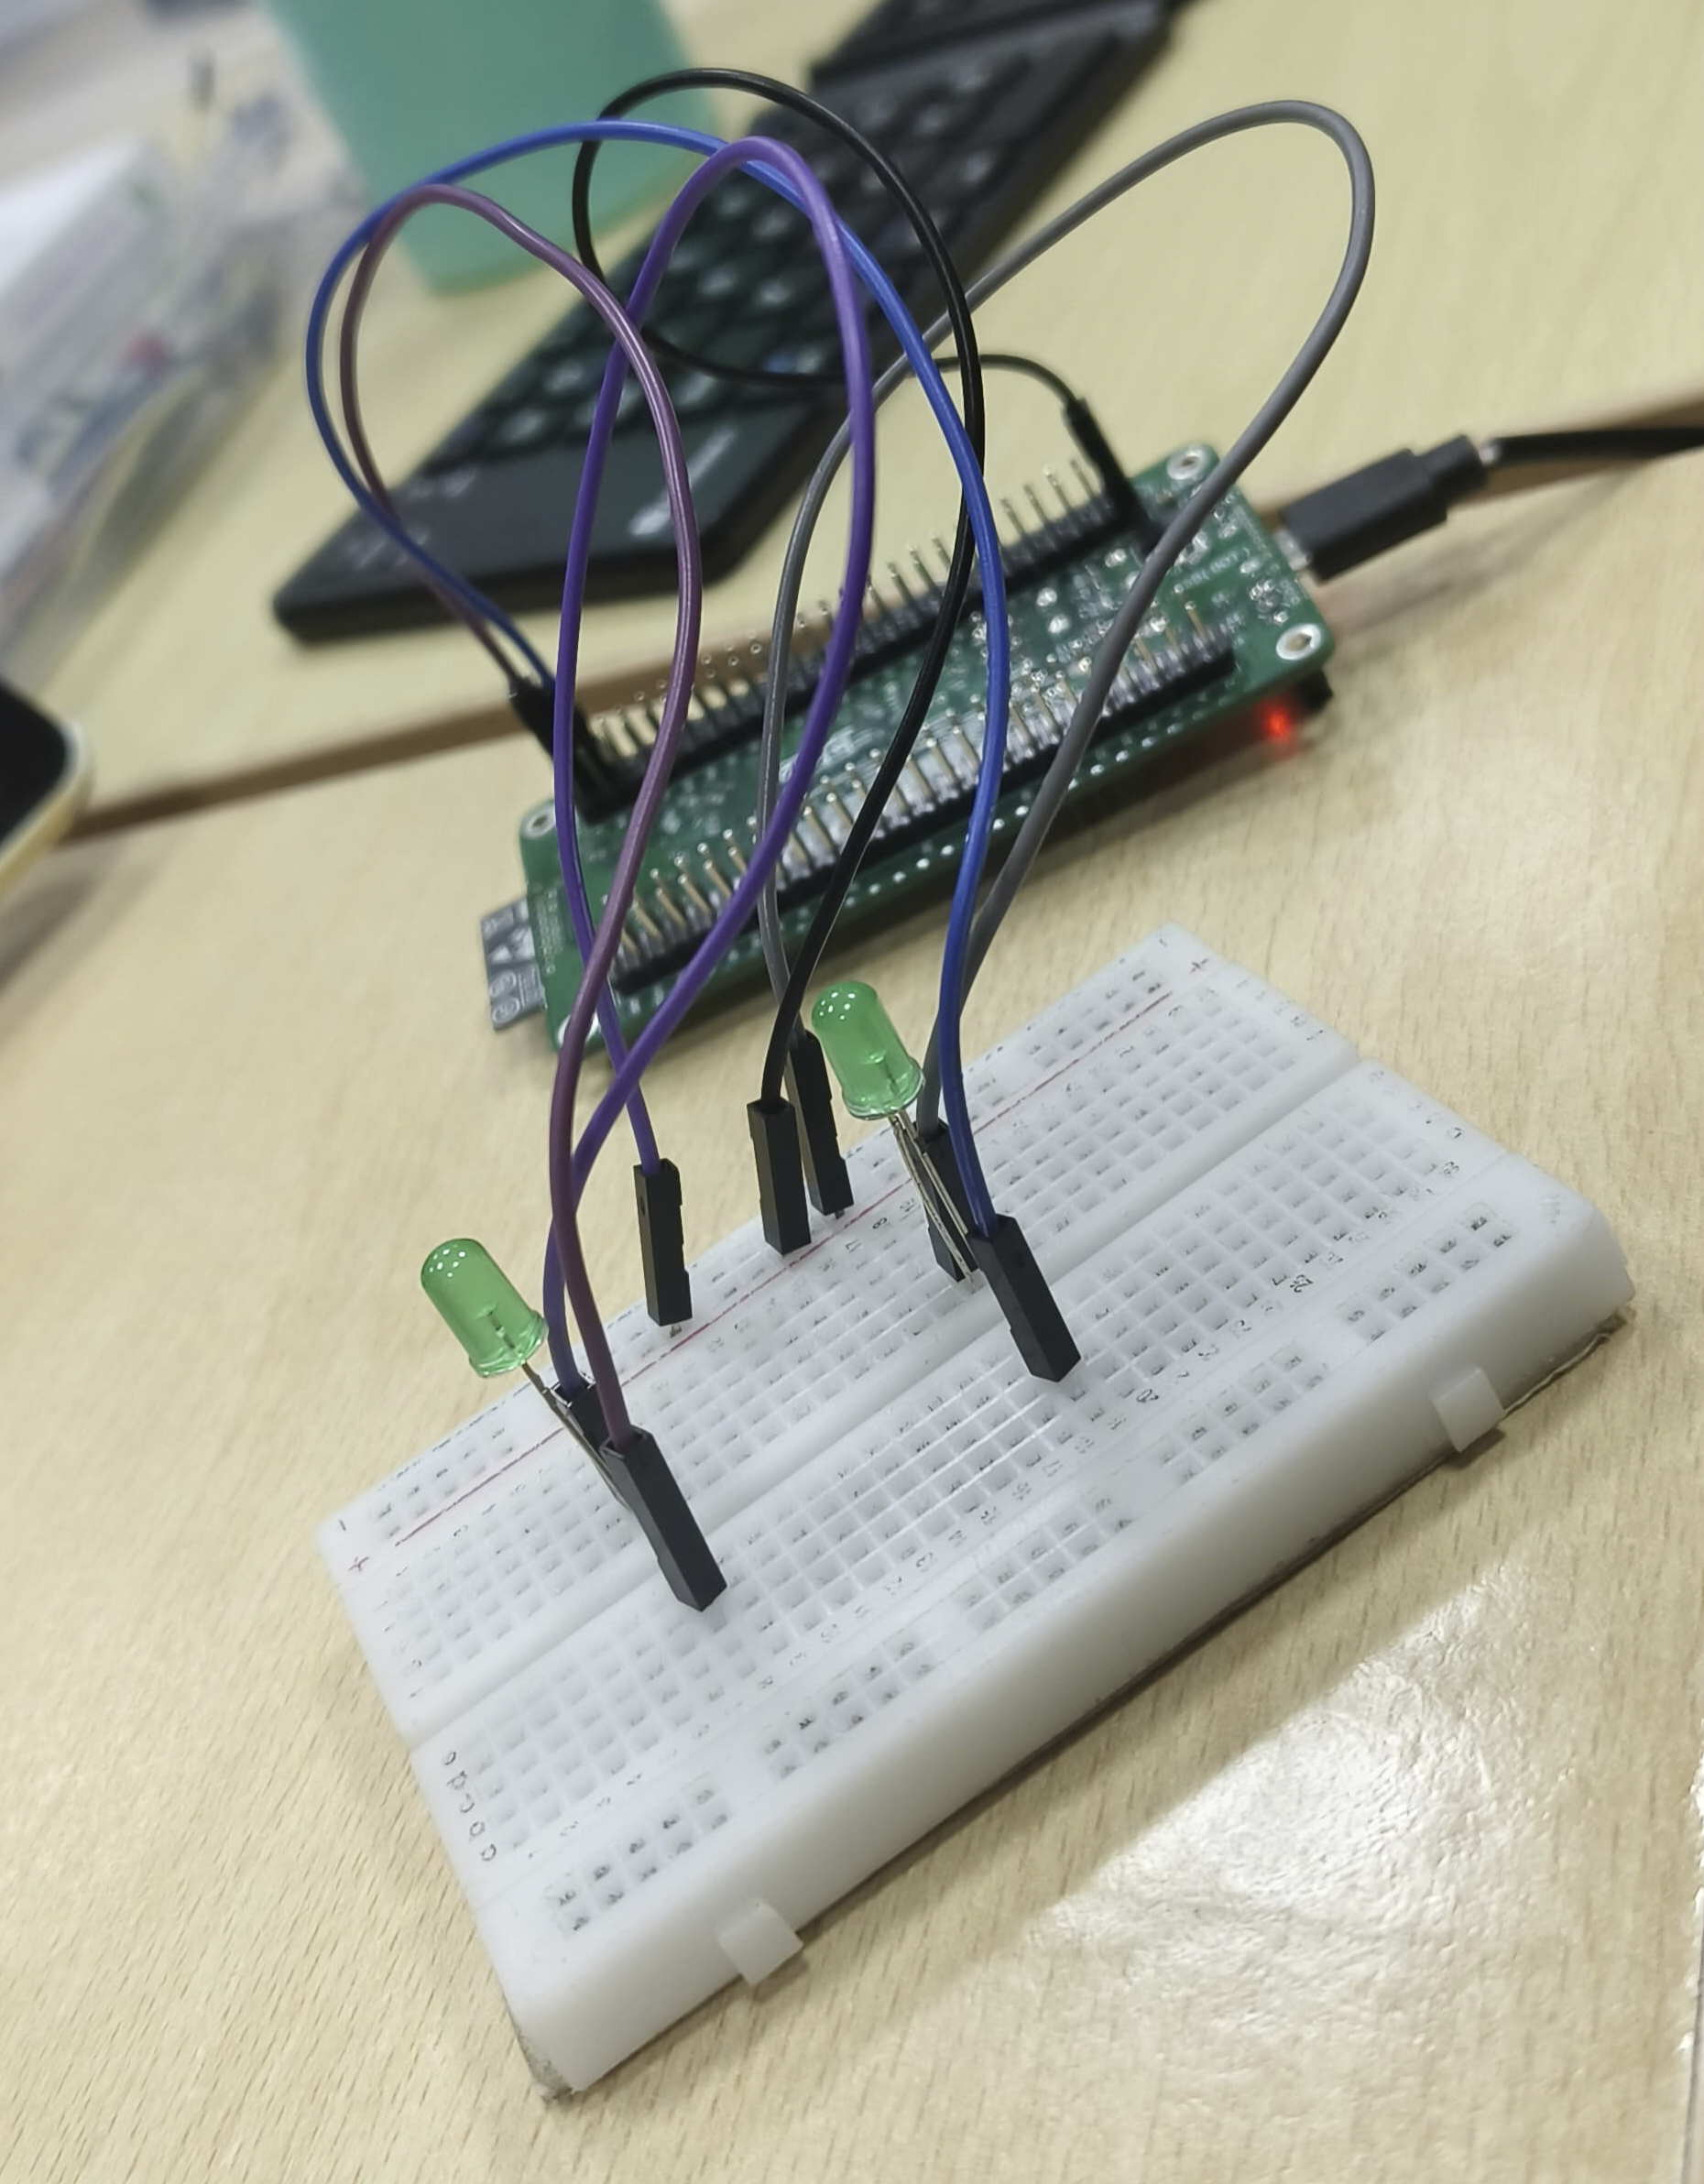
\includegraphics[width=0.3\textwidth]{	/storage/emulated/0/vignan/IMG_20241028_125918.jpg}                                
\caption{\label{fig-5:Gates}}             
\end{figure}




 \begin{figure}[h]                           
\centering                                 
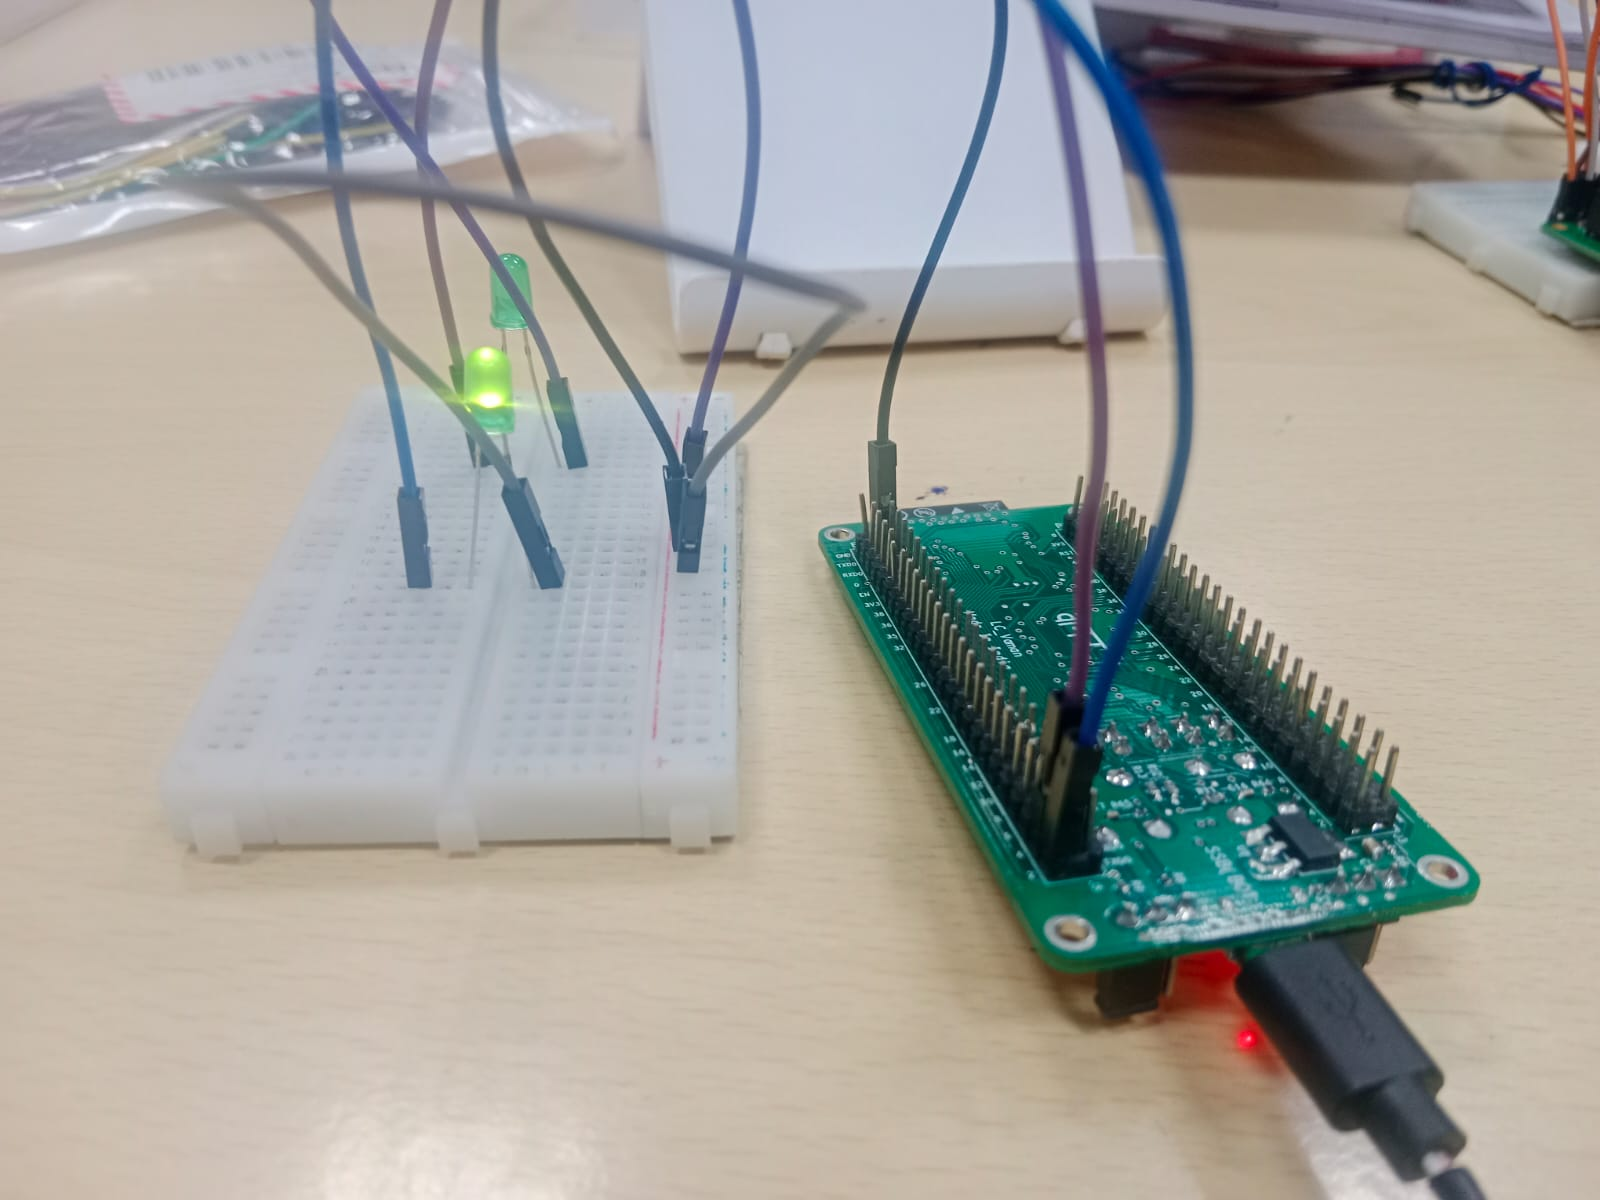
\includegraphics[width=0.35\textwidth]{ /storage/emulated/0/vignan/IMG-20241028-WA0002.jpg}                                           
\caption{\label{fig-6:Gates}}               
\end{figure}
\section{CONCLUSION}
Hence implementation of above astract using esp code with vaman board and verification through leds is done .


\end{document}
